% Composites the final 4-panel manuscript Figure 1 from independently
% generated sub-panel PDFs/PNGs. Run: pdflatex -interaction=nonstopmode compose_figure1.tex
% Panel sources:
%   A = figure1_out/panel_C_actb.pdf        (panel_C_integration.py ptprc/actb)
%   B = figure1_out/panel_C_ptprc.pdf       (panel_C_integration.py ptprc)
%   C = figure1_out/panel_E_distribution.pdf (panel_E_distribution.py)
%   D = three volcano PNGs from ../../results_all_bams/*/plots_capped/
\documentclass[preview,border=4pt]{standalone}
\usepackage{graphicx}
\setlength{\parindent}{0pt}
\begin{document}
\begin{minipage}{7.4in}

\noindent
\begin{minipage}[t]{0.49\linewidth}
\textbf{\Large A}\par\vspace{2pt}
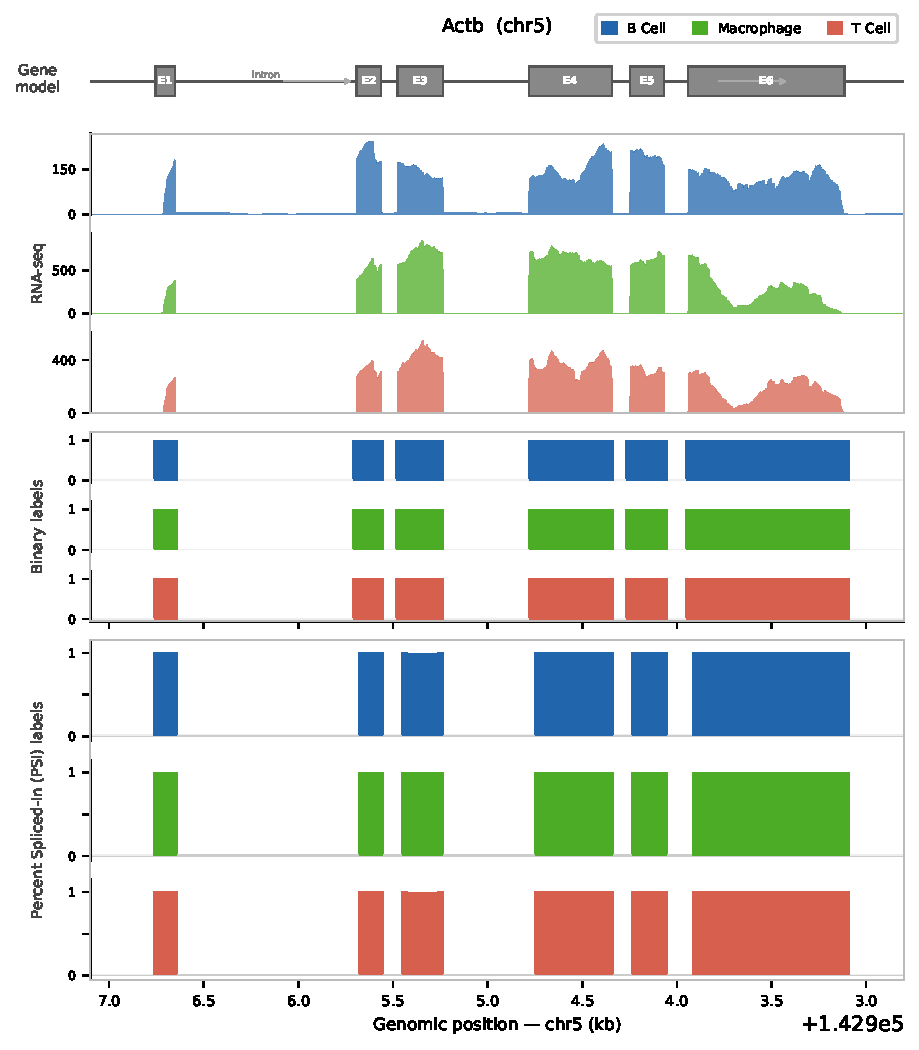
\includegraphics[width=\linewidth]{figure1_out/panel_C_actb.pdf}
\end{minipage}%
\hfill
\begin{minipage}[t]{0.49\linewidth}
\textbf{\Large B}\par\vspace{2pt}
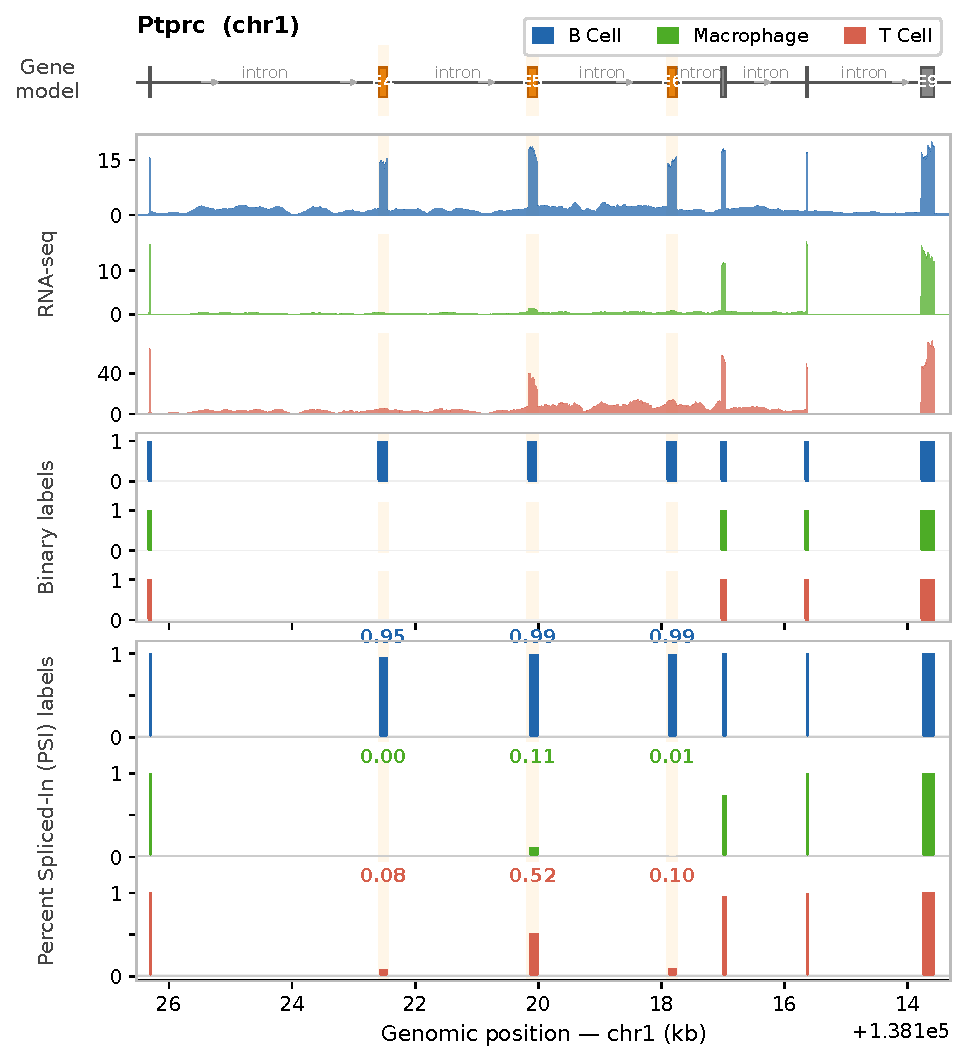
\includegraphics[width=\linewidth]{figure1_out/panel_C_ptprc.pdf}
\end{minipage}

\vspace{10pt}

\textbf{\Large C}\par\vspace{2pt}
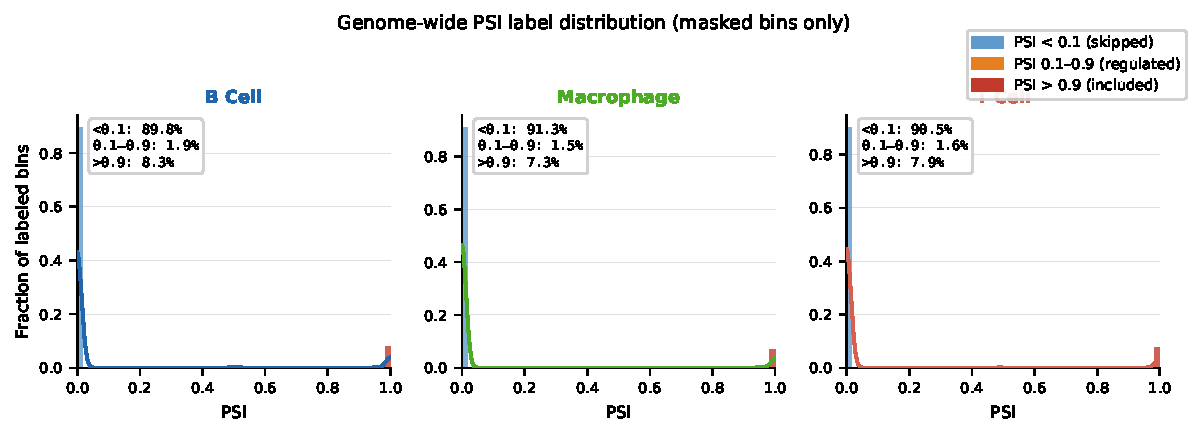
\includegraphics[width=\linewidth]{figure1_out/panel_E_distribution.pdf}

\vspace{10pt}

\textbf{\Large D}\par\vspace{2pt}
\begin{minipage}[t]{0.327\linewidth}
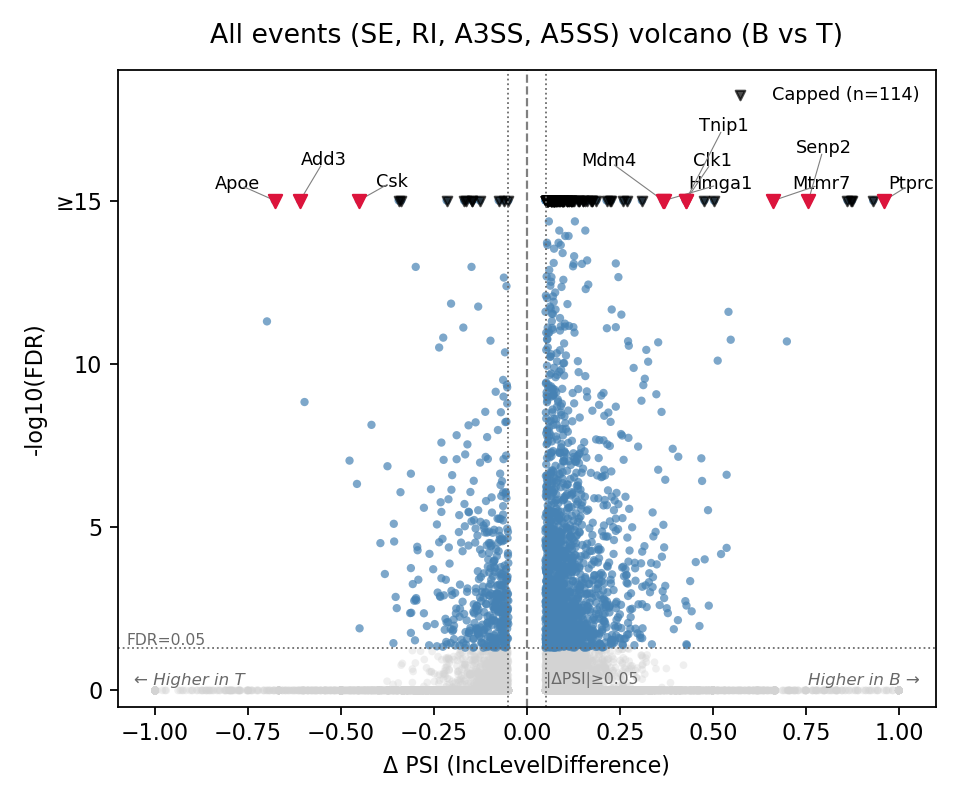
\includegraphics[width=\linewidth]{../../results_all_bams/B_vs_T/plots_capped/B_vs_T_all_events_volcano.png}
\end{minipage}%
\hfill
\begin{minipage}[t]{0.327\linewidth}
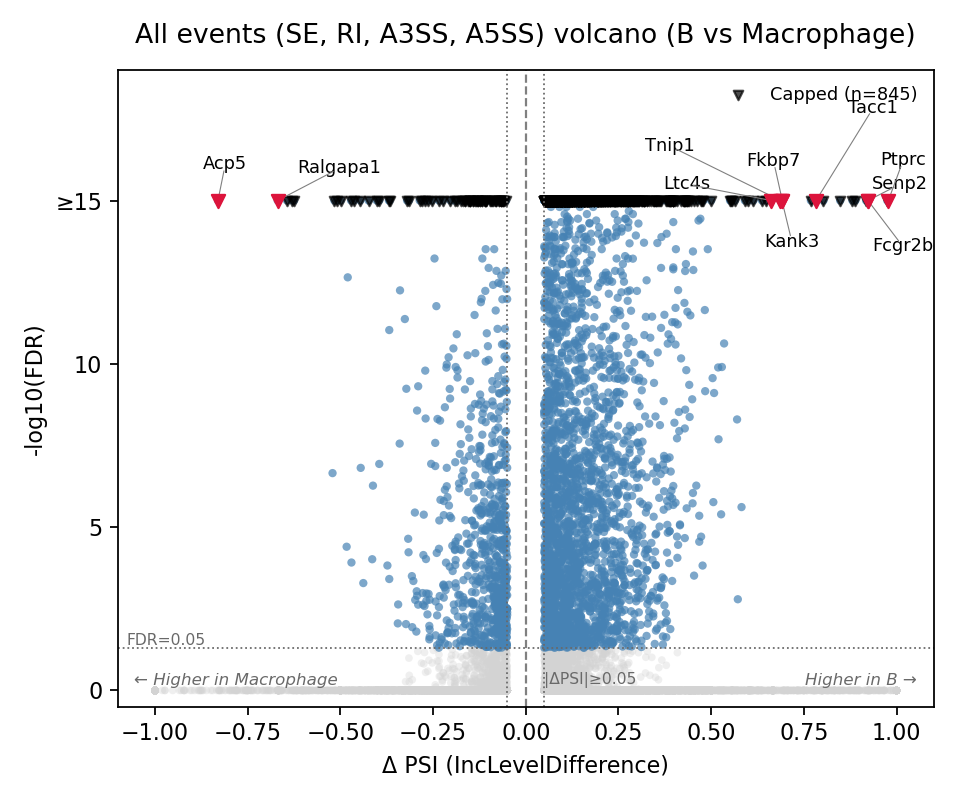
\includegraphics[width=\linewidth]{../../results_all_bams/B_vs_Macrophage/plots_capped/B_vs_Macrophage_all_events_volcano.png}
\end{minipage}%
\hfill
\begin{minipage}[t]{0.327\linewidth}
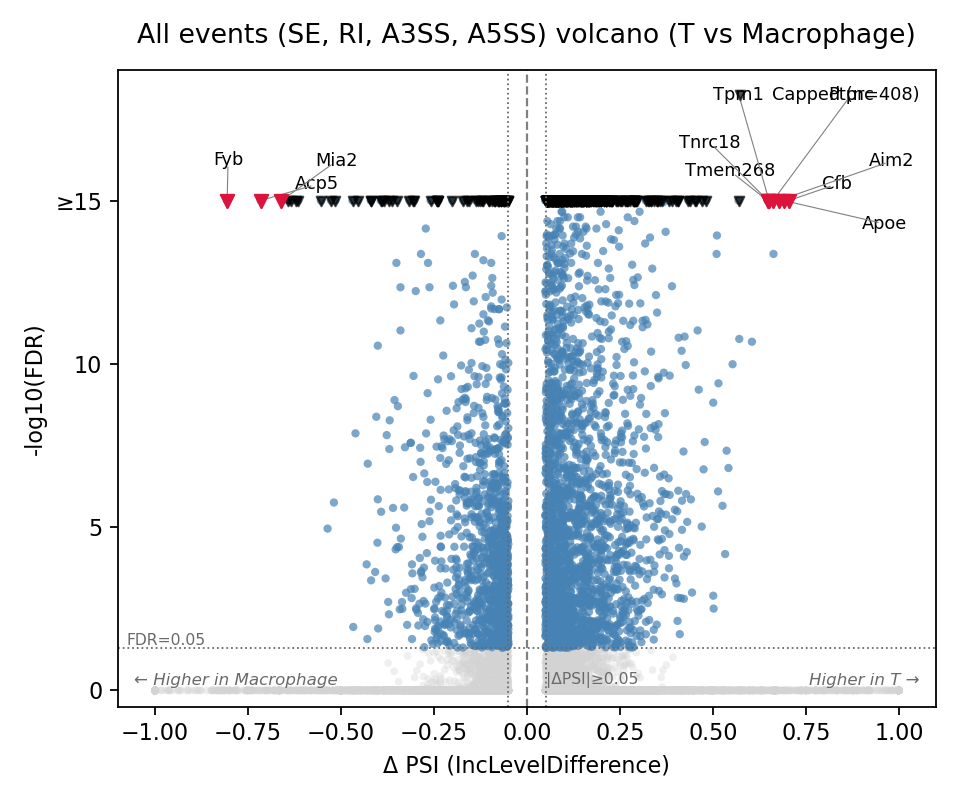
\includegraphics[width=\linewidth]{../../results_all_bams/T_vs_Macrophage/plots_capped/T_vs_Macrophage_all_events_volcano.png}
\end{minipage}

\end{minipage}
\end{document}
